\chapter{Geometria Analitica}

\section{Noções Iniciais}
\subsection{Distância Entre Dois Pontos}

Dados dois pontos $A(x_a\, , y_a)$ e $B(x_b\, , y_b)$ a distância entre $A$ e $B$ é dada por:
$$d_{AB} = \sqrt{(x_a - x_b)^2 + (y_a - y_b)^2}$$


\begin{figure}[H]
	\centering
	
	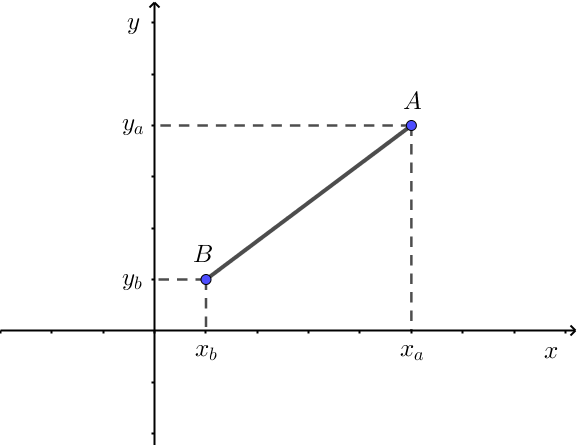
\includegraphics[scale=3.5]{imagens/distanciaab.png}

\end{figure}

\newtheorem{proof}{Demonstração}
\begin{proof}
Vamos demonstrar a formula da distância entre dois pontos.
Considere o triângulo $ABC$ na imagem abaixo:
\end{proof}

\begin{figure}[H]
	\centering
	
	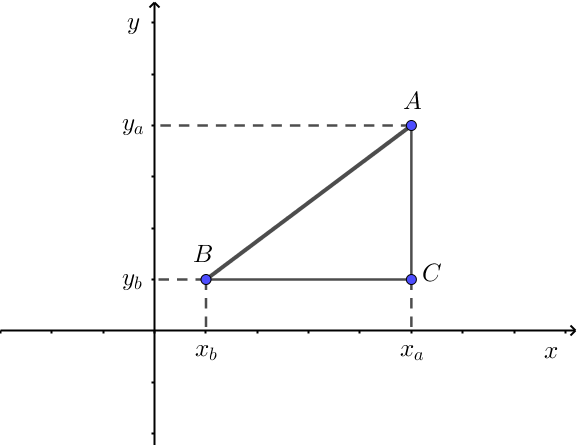
\includegraphics[scale=3.5]{imagens/distanciad.png}

\end{figure}
\begin{center}
Aplicando o teorema de Pitágoras no triângulo $ABC$ temos:
\end{center}


$$d_{AB}^2 = d_{BC}^2 + d_{AC}^2$$
\begin{center}
Do triângulo $ABC$ temos  que $d_{BC} = (x_a - x_b)$ e $d_{AC} = (y_a - y_b)$ então:
\end{center}

$$d_{AB}^2 ={(x_a - x_b)}^2 + {(y_a - y_b)}^2   $$

$$d_{AB} = \sqrt{{(x_a - x_b)}^2 + {(y_a - y_b)}^2}$$


\subsection{Circunferência}

Uma circunferência é o conjunto de pontos no plano que estão a uma certa distância $r$ de um ponto dado $( a, b )$.
Um ponto $( x, y )$ pertence a circunferência
de centro $( a, b )$ e raio $r$ se e somente se satisfaz a equação:

$${(x - a)}^2 + {(y - b)}^2=r^2$$
\begin{figure}[H]
	\centering
	
	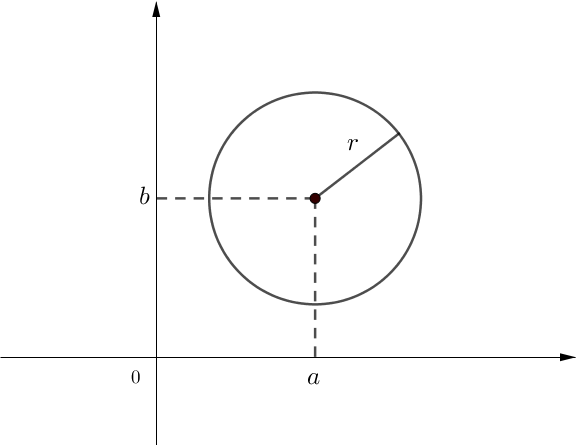
\includegraphics[scale=3.5]{imagens/circunferencia1.png}

\end{figure}
\newtheorem{proof}{Demonstração}
\begin{proof}
Vamos demonstrar a equação da circunferência.
Considere a seguinte imagem abaixo:
\end{proof}

\begin{figure}[H]
	\centering
	
	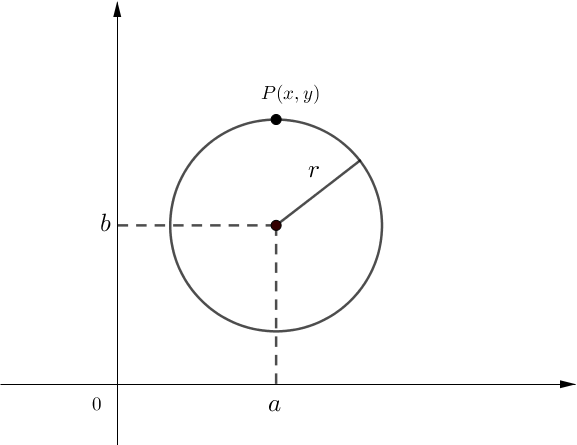
\includegraphics[scale=3.5]{imagens/circunferencia2.png}

\end{figure}
\begin{center}
Usando a definição de circunferência, temos que um ponto $P(x,y)$ pertence a circunferência se e somente se a distância dele até o centro $C(a,b)$ é igual a $r$. Escrevendo essa relação, temos:
\end{center}

$$ d_{PC} = r $$

\begin{center}

Usando a equação da distância entre dois pontos e substituindo na equação acima, temos:

\end{center}
$$\sqrt{{(x - a)}^2 + {(y - b)}^2} = r $$

\begin{center}

elevando ao quadrado os dois lados da equação acima, temos:

\end{center}

$$ {(x - a)}^2 + {(y - b)}^2 = r^2$$